% Relatório de EXEMPLO — pipeline completo com dados reais (facções na Amazônia Legal)
\documentclass[10pt,a4paper,twocolumn]{article}
\usepackage[utf8]{inputenc}
\usepackage[T1]{fontenc}
\usepackage{lmodern}
\usepackage[brazilian]{babel}
\usepackage[margin=2cm]{geometry}
\usepackage{graphicx,booktabs,amsmath,hyperref}

\title{Do Simbólico à Incerteza: inferindo a presença e a expansão de facções criminosas nos municípios da Amazônia Legal\\
\large (exemplo didático do pipeline com dados reais)}
\author{Equipe — Fundamentos de Inteligência Artificial (IComp/UFAM)}
\date{\today}

\begin{document}
\maketitle

\begin{abstract}
A presença de facções criminosas não aparece em nenhuma base oficial: é uma variável oculta.
Combinamos as estatísticas de violência do SINESP VDE (2020--2023) e a população do IBGE para
inferi-la nos 808 municípios dos estados da Amazônia Legal, usando como referência o
\emph{Cartografias da Violência na Amazônia} de 2024. A rede bayesiana diagnóstica atinge
AUC de 0,81. Sem usar nenhum dado de 2025, a probabilidade calculada antecipa quais municípios
passaram a ter facção segundo a edição de 2025 (AUC 0,76): na prioridade fuzzy baixa, 13\%
entraram; na alta, 44\%.
\end{abstract}

\section{Introdução e dados}
% TODO: contexto da expansão de facções na Amazônia (Cartografias; Siqueira e Paiva 2019; Sales et al. 2025).
Rótulos: \emph{Cartografias da Violência na Amazônia}, 3ª edição (259 municípios com facção em
2024) e 4ª edição (344 em 2025, quadros extraídos do PDF). Atributos: Banco VDE do Ministério da
Justiça. População: IBGE (Censo 2022), unida pelo código IBGE. Todos os 5.570 municípios do VDE
casaram com o IBGE pelo nome.

\section{Etapa 1 — Árvore de decisão}
Entropia na raiz: 0,905 bits. Maiores ganhos: porte (0,165) e UF (0,151); as taxas de violência
vêm bem depois (0,027).
% TODO: colar os 3 primeiros níveis (saída de "detalhar").
\begin{table}[h]\centering\small
\begin{tabular}{lccc}\toprule
Modelo & Treino & Teste & Bal.\\\midrule
ID3 própria, sem poda & 0,874 & 0,749 & 0,687\\
ID3 própria, prof. 3 & 0,824 & 0,786 & 0,708\\
sklearn, prof. 4 & 0,799 & 0,782 & 0,679\\\bottomrule
\end{tabular}\caption{Validação cruzada 5-fold; os tercis das taxas são calculados só com o treino de cada dobra.}\end{table}

\textbf{Monotonicidade.} A regra ``município pequeno $\Rightarrow$ sem facção'' cobre 267
municípios e acerta 89,9\%. Acrescentando o fato ``fica no Acre'' ou ``em Roraima'', a conclusão
se inverte: todos os pequenos desses estados têm facção.

\section{Etapa 2 — Modelos lineares}
\begin{table}[h]\centering\small
\begin{tabular}{lcc}\toprule
Modelo & $R^2$ & Acurácia (bal.)\\\midrule
Simples (hom. 2022 $\to$ 2023) & 0,672 & --\\
Multivariada (GD, 16 atributos) & 0,763 & --\\
Ridge ($\lambda=0{,}084$) & 0,762 & --\\
Logística (facção) & -- & 0,759 (0,737)\\\bottomrule
\end{tabular}\caption{Teste (20\%). O scikit-learn dá os mesmos valores.}\end{table}

\section{Etapa 3 — Probabilidade}
Com a taxa por 100 mil, $P(F\mid V)=0{,}424$ contra $0{,}269$ (1,6 vez); a contagem bruta exagerava
o sinal porque misturava tamanho. A regra da cadeia confere nos 8 eventos.
\textbf{Transições:} dos 549 municípios sem registro em 2024, 129 (23,5\%) passaram a ter facção
em 2025; a chance cresce com o porte (14\% nos pequenos, 37\% nos grandes). 16 municípios
passaram de domínio para disputa, e 45 ``saíram'' da lista, o que sugere mudança de método.

\section{Etapa 4 — MLE, MAP, Naive Bayes e EM}
No Acre, $\hat\theta_{MLE}=1{,}0$ e $\hat\theta_{MAP}=0{,}958$. O Naive Bayes do zero acerta
77,2\% (0,737 balanceada). O EM com $K=3$ na contagem de homicídios produz grupos que acompanham
o Cartografias (1,7\% em disputa no grupo menos violento, 29\% no mais violento). Com a taxa, a
correspondência é mais fraca: a facção está ligada ao volume de violência, não só à intensidade.
Foi preciso um piso de variância para evitar o colapso da componente dos municípios sem homicídio.

\section{Etapa 5 — Rede bayesiana}
DAG: \texttt{PORTE}$\to$\texttt{FACCAO}$\leftarrow$\texttt{FRONT};
\texttt{FACCAO}$\to$\{\texttt{TXH}, \texttt{ESC}, \texttt{TXT}\}. São 19 parâmetros contra 215
(91\% de economia). A enumeração coincide com o \texttt{pgmpy}. \textbf{Colisor:} sem observar a
facção, porte e fronteira são independentes; dado que há facção, ser pequeno eleva
$P(\text{fronteira})$ de 0,61 (grande) para 0,96. Nos dados, porte e fronteira têm correlação 0,21:
a suposição é aproximada. Como classificador, a rede tem AUC de 0,81.

\textbf{Validação geográfica.} Treinando com 8 estados e testando no 9º, a AUC geral fica em 0,80.
A rede ordena bem os municípios em TO (0,94), AP, MA e PA, mas mal em RO (0,58), RR e AM, e erra o
\emph{nível} onde a facção é quase universal: no Acre (100\%) e em Roraima (93\%) a probabilidade
média prevista é cerca de 0,47, porque \texttt{FRONT} só distingue MA e TO dos demais estados.
A rede serve para ordenar municípios num estado conhecido, não para estimar o nível num estado novo.

\textbf{Sensibilidade ao rótulo.} Sem os 45 municípios que ``saíram'' da lista em 2025, a AUC sobe para
0,83; a rede já os via com probabilidade intermediária (0,40, contra 0,58 dos que têm facção nas duas
edições), o que sugere erro de registro ou mudança de método. Com o rótulo ``facção em 2024 ou 2025'',
a AUC é 0,82. As conclusões não dependem do ruído do rótulo.

\section{Etapa 6 — Fuzzy, integração e validação com 2025}
\begin{table}[h]\centering\small
\begin{tabular}{lccc}\toprule
Prioridade & Munic. & Facção 2024 & Entrada 2025$^*$\\\midrule
Baixa & 404 & 12,9\% & 13,1\%\\
Média & 165 & 37,6\% & 40,8\%\\
Alta & 239 & 60,7\% & 43,6\%\\\bottomrule
\end{tabular}\caption{$^*$Entre os municípios sem facção em 2024. AUC da probabilidade bayesiana
para prever a entrada: 0,764 (probabilidades fora da dobra).}\end{table}
\textbf{Com os dados de 2024.} Trocar os atributos de 2021--23 por 2022--24 não melhora a previsão da
entrada em 2025 (AUC 0,754 nas duas janelas). Municípios com salto de homicídios em 2024 entraram
mais (31\% contra 21\%), mas o salto de 2023 tem o mesmo efeito (32\% contra 21\%): é sinal de
município violento, não da chegada da facção. O padrão de Iranduba não se confirma na escala regional.
\begin{figure}[h]\centering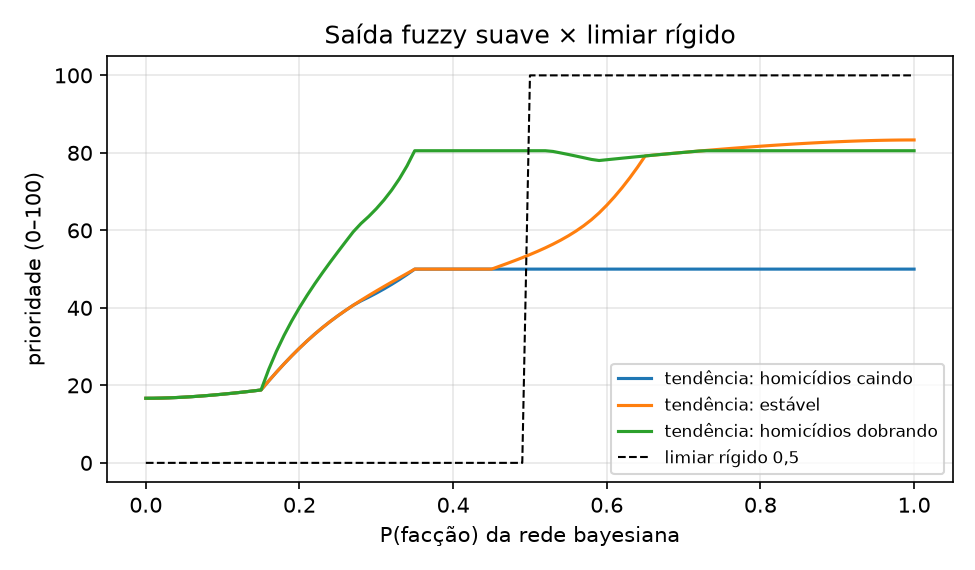
\includegraphics[width=\columnwidth]{../figuras/etapa6_fuzzy_vs_rigido.png}
\caption{Saída fuzzy suave × limiar rígido.}\end{figure}

\section{Conclusão e limitações}
% TODO: "sem registro" não é ausência certa; mudanças entre edições refletem também o método;
% a violência indica onde, não quando (teste da janela 2022--24 e do salto de 2024);
% divergências internas do relatório (AP, PA, TO); MA entra inteiro; ética de rotular municípios;
% FRONT por estado: a rede não acerta o nível de facção num estado que não viu (AC, RR).

\begin{thebibliography}{9}
\bibitem{aima} S. Russell e P. Norvig. \emph{Artificial Intelligence: A Modern Approach}, 4. ed. Pearson, 2020.
\bibitem{carto3} Instituto Mãe Crioula e FBSP. \emph{Cartografias da Violência na Amazônia}, 3. ed., 2024.
\bibitem{carto4} Instituto Mãe Crioula e FBSP. \emph{Cartografias da Violência na Amazônia}, 4. ed., 2025.
\bibitem{vde} Ministério da Justiça e Segurança Pública. Banco VDE (SINESP), 2020--2024. Acesso em out. 2026.
\bibitem{ibge} IBGE. Censo Demográfico 2022 e Estimativas da População. Acesso em nov. 2026.
\bibitem{siq} I. Siqueira e L. Paiva. ``No Norte, tem Comando''. \emph{Rev. Bras. Sociologia}, v. 7, n. 17, 2019.
\bibitem{ribeiro} J. Ribeiro et al. Prediction of Homicides in Urban Centers. arXiv:2008.06979.
\end{thebibliography}
\end{document}
